\documentclass[main.tex]{subfiles}
\newcommand\chapterlabel{Ch-kinetics}\setcounter{figurenewcounter}{0}\setcounter{tablenewcounter}{0}\setcounter{formulanewcounter}{0}\chapterpicture{../{\chapterlabel}/figure1}\chapterpicturelabel{PxFuel}
\setcounter{figurenewcounter}{0}




 
\begin{document}
%\setcounter{chapter}{5}
  
 
 \setcounter{chapter}{2}  \import{../\chapterlabel/files/}{ChapterName}


%\label{ch:atoms}

%
%      \begin{marginfigure}
%      \begin{tikzpicture} \node (a) at (0,0) {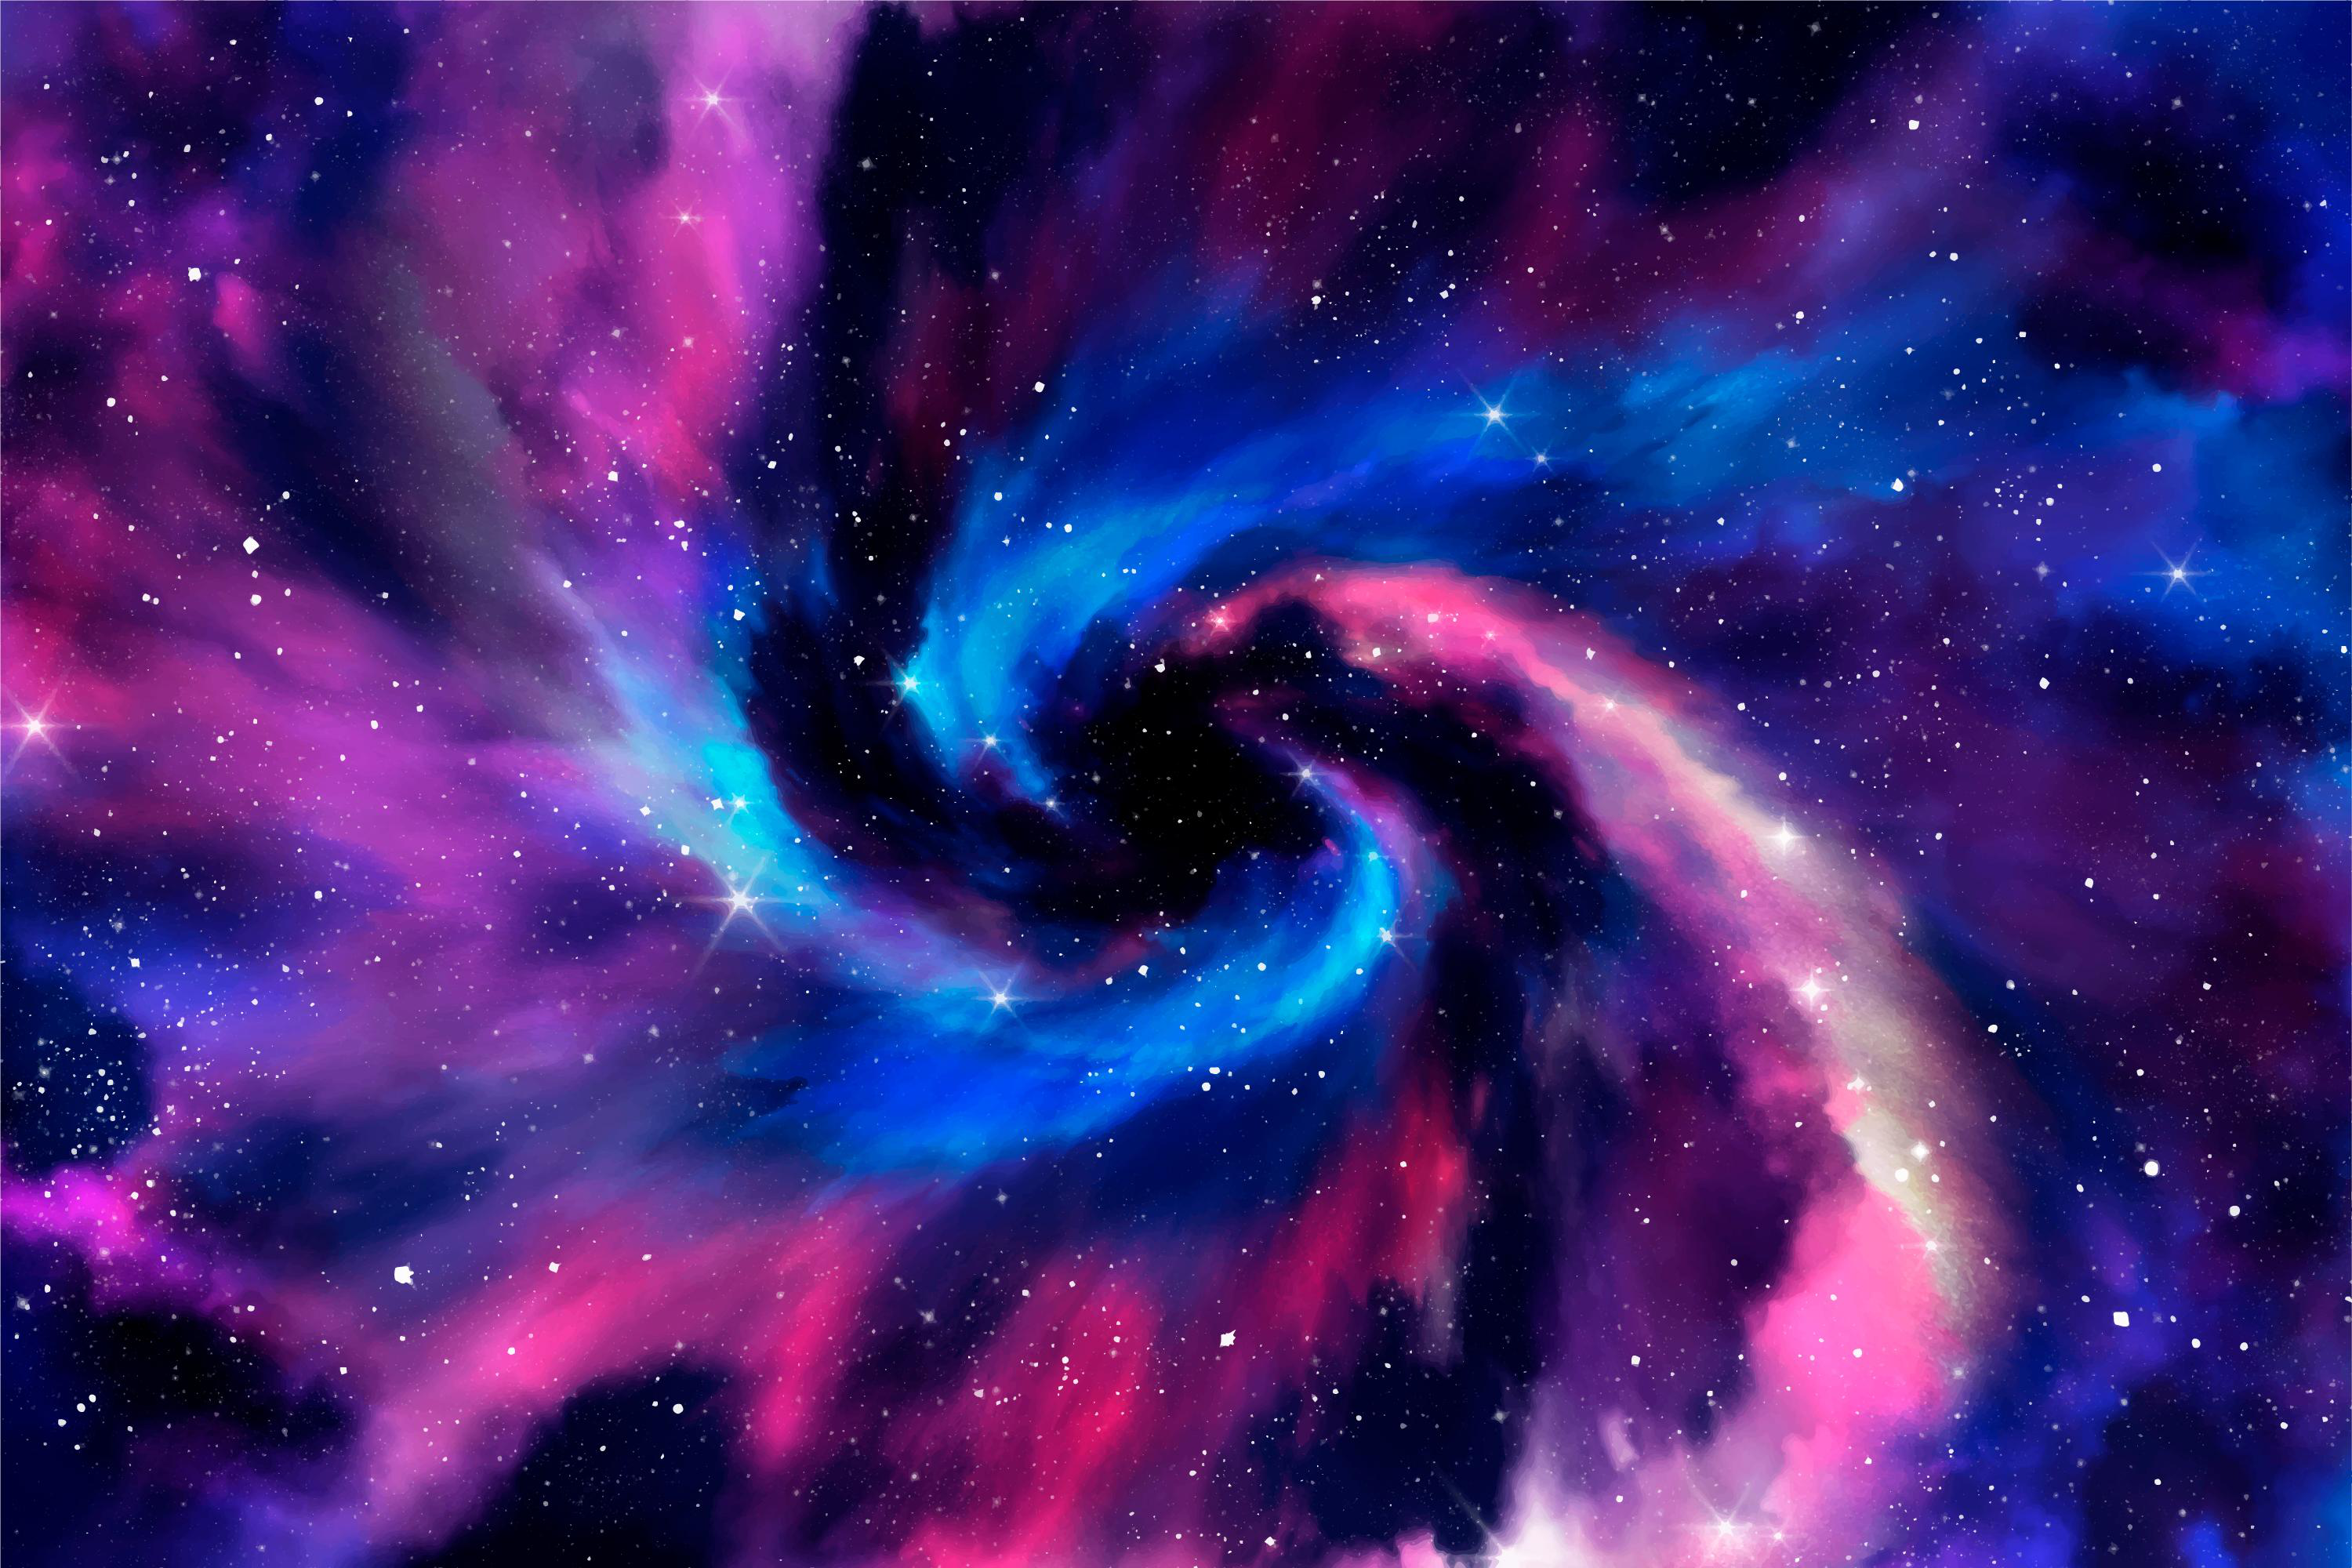
\includegraphics[width=4cm]{../Ch-kinetics/figure1}} node[rotate=90, font=\tiny] at ([yshift=.5cm,xshift=.1cm]a.south east) {\textsuperscript{\textcopyright} PxFuel} ;
%\end{tikzpicture}
%\end{marginfigure}
  \import{../\chapterlabel/files/}{ChapterIntro}



%\begin{marginfigure}%LEARNING GOALS BOX
%\begin{mytcbox}{GOALS}
%\begin{enumerate}[label=\protect\circled{\color{white}\arabic*}]
%\item Analyze a rate law
%\item Interconvert rates of reactants and products
%\item Obtain rate laws
%\item Compute activation energies
%\item Analyze energy profiles
%\end{enumerate}
%\end{mytcbox}
%\vspace{1cm}
%\begin{tcolorbox}[enhanced,colback=red!5!white,colframe=black!50!red,boxrule=1pt,
%  arc=0pt,outer arc=0pt,drop heavy lifted shadow]
%\faGears\ 
%\docenvdef{Discussion:} (a) \discussionKINETICSA (b) \discussionKINETICS \end{tcolorbox}
%\end{marginfigure}%LEARNING GOALS BOX




\section{Rate of reaction}\import{../\chapterlabel/files/}{SectionIntro-Rate-of-reaction}
\sloppy\begin{description}
\item[\docfilehook{Two different ways of defining the reaction rate}{}] \import{../\chapterlabel/files/}{Section-Rate-of-reaction-Subsection-Two-different-ways-of-defining-the-reaction-rate}
%\Adddocfilehookr{



  \import{../\chapterlabel/files/}{Figure-c-vs-t}
\item[\docfilehook{Rate of appearance and disappearance}{}] \import{../\chapterlabel/files/}{Section-Rate-of-reaction-Subsection-Rate-of-appearance-and-disappearance}
\end{description}

  \import{../\chapterlabel/problems/}{SampleProblem1}
  \import{../\chapterlabel/files/}{Figure-fast-and-slow}

\section{Rate law}\import{../\chapterlabel/files/}{SectionIntro-Rate-law}
 \sloppy \begin{description}
\item[\docfilehook{The rate law}{}] \import{../\chapterlabel/files/}{Section-Rate-of-reaction-Subsection-The-rate-law}
\item[\docfilehook{Partial and overall reaction orders}{}] \import{../\chapterlabel/files/}{Section-Rate-of-reaction-Subsection-Partial-and-overall-reaction-orders}
\item[\docfilehook{The rate constant, k}{}] \import{../\chapterlabel/files/}{Section-Rate-of-reaction-Subsection-The-rate-constant-k}
\import{../\chapterlabel/problems/}{SampleProblem2}
\item[\docfilehook{The rate constant units}{}] \import{../\chapterlabel/files/}{Section-Rate-of-reaction-Subsection-The-rate-constant-units}
\import{../\chapterlabel/problems/}{SampleProblem3}
\item[\docfilehook{Integral reaction law}{}] \import{../\chapterlabel/files/}{Section-Rate-of-reaction-Subsection-Integral-reaction-law}
\import{../\chapterlabel/files/}{Table-integral-formulas}
\import{../\chapterlabel/problems/}{SampleProblem4}
\item[\docfilehook{Half-life, $t_{\nicefrac{1}{2}}$}{}]  \import{../\chapterlabel/files/}{Section-Rate-of-reaction-Subsection-Half-life}
\end{description}
\import{../\chapterlabel/problems/}{SampleProblem5}



\section{The differential and integral methods for obtaining rate laws}\import{../\chapterlabel/files/}{SectionIntro-Dif-and-integral}
\sloppy \begin{description}
\item[\docfilehook{The differential method}{}] \import{../\chapterlabel/files/}{SectionIntro-Dif-and-integralSubsection-The-differential-method}
  \import{../\chapterlabel/problems/}{SampleProblem6}
\item[\docfilehook{The differential method with two reactants}{}] \import{../\chapterlabel/files/}{SectionIntro-Dif-and-integralSubsection-The-differential-method-two}
  \import{../\chapterlabel/problems/}{SampleProblem7}
  \import{../\chapterlabel/files/}{Table-the-integral-method}
 \item[\docfilehook{The integral method: an introduction}{}] \import{../\chapterlabel/files/}{SectionIntro-Dif-and-integralSubsection-The-integral-method-an-introduction}
\item[\docfilehook{The integral method: associating a linear plot with an order}{}] \import{../\chapterlabel/files/}{SectionIntro-Dif-and-integralSubsection-The-integral-method-associating-a-linear-plot-with-an-order}
  \import{../\chapterlabel/problems/}{SampleProblem8}
\item[\docfilehook{The integral method: extracting data from linear regressions}{}] \import{../\chapterlabel/files/}{SectionIntro-Dif-and-integralSubsection-The-integral-method-extracting-data-from-linear-regressions}
  \import{../\chapterlabel/problems/}{SampleProblem9}
  \import{../\chapterlabel/problems/}{SampleProblem10}
\item[\docfilehook{The integral method in action}{}] \import{../\chapterlabel/files/}{SectionIntro-Dif-and-integralSubsection-The-integral-method-in-action}
\item[\docfilehook{The integral method for more than one reactant}{}] \import{../\chapterlabel/files/}{SectionIntro-Dif-and-integralSubsection-The-integral-method-for-more-than-one-reactant}
\end{description}
  \import{../\chapterlabel/files/}{Figure-energy-diagram1}




\section{\color{blue!30!black}{Collision theory}}\import{../\chapterlabel/files/}{SectionIntro-Collision-theory}
\sloppy \begin{description}
\item[\docfilehook{Collision theory}{}] \import{../\chapterlabel/files/}{Subsecion-Collision-theory}
\item[\docfilehook{Transition state and activation energy}{}]\import{../\chapterlabel/files/}{Subsecion-Transition-state-and-activation-energy} 
\import{../\chapterlabel/files/}{Figure-Transition-state-two-paths} 
\item[\docfilehook{Effect of temperature}{}] \import{../\chapterlabel/files/}{Subsecion-Effect-of-temperature} 
\item[\docfilehook{Concentration of reactants}{}] \import{../\chapterlabel/files/}{Subsecion-Concentration-of-reactants}
\import{../\chapterlabel/problems/}{SampleProblem11}
 \vspace{1cm}  \import{../\chapterlabel/files/}{Figure-Collision-theory} \newpage
\item[\docfilehook{Catalysts}{}] \import{../\chapterlabel/files/}{Subsecion-Catalyst}
\import{../\chapterlabel/files/}{Figure-Energy-profile-catalys}  
\item[\docfilehook{Heterogeneous catalysis}{}] \import{../\chapterlabel/files/}{Subsecion-Hetero-Catalyst}
\import{../\chapterlabel/files/}{Figure-catalyst-mechanism-steps}  
\end{description}

 

\section{Use of energy diagrams}
\sloppy \begin{description}
\item[\docfilehook{Energy diagrams}{}] \import{../\chapterlabel/files/}{Subsecion-Energy-diagrams}
  \import{../\chapterlabel/problems/}{SampleProblem12}
  \import{../\chapterlabel/files/}{Figure-set-of-energy-profiles}
\end{description}


\section{The Arrhenius equation}
\sloppy \begin{description}
\item[\docfilehook{The Arrhenius equation on its exponential form}{}] \import{../\chapterlabel/files/}{SubsectionThe-Arrhenius-equation-on-its-exponential-form}
  \import{../\chapterlabel/problems/}{SampleProblem13}
  \import{../\chapterlabel/problems/}{SampleProblem14}
\end{description}



\section{Reaction mechanisms} \import{../\chapterlabel/files/}{SectionIntro-Reaction-mechanisms}
\sloppy \begin{description}
\item[\docfilehook{An example of a reaction mechanism}{}]  \import{../\chapterlabel/files/}{SectionIntro-Reaction-mechanismsSubsectionAn-example-of-a-reaction-mechanism}
\item[\docfilehook{Rate limiting step}{}] \import{../\chapterlabel/files/}{SectionIntro-Reaction-mechanismsSubsectionRate-limiting-step}
\item[\docfilehook{Equilibrated steps }{}] \import{../\chapterlabel/files/}{SectionIntro-Reaction-mechanismsSubsectionEq-step}
 \item[\docfilehook{How to verify a possible mechanism }{}] \import{../\chapterlabel/files/}{SectionIntro-Reaction-mechanismsSubsectionHow-to-verify-a-possible-mechanism}
  \import{../\chapterlabel/problems/}{SampleProblem15}
  \end{description}



\checkoddpage\ifoddpage \clearpage\thispagestyle{empty}\mbox{}\clearpage \else  \fi \end{document}

